\chapter{Descrizione del problema}
\label{chap:3}
    
    \paragraph{Medical Image Analysis}
    L'analisi delle immagini mediche ha lo scopo di esaminare il corpo umano per motivi medici come la diagnosi, i trattamenti e il monitoraggio della salute. Con il passare degli anni le DNN si sono rivelate la scelta migliore per trattare dati complessi e ad alta dimensione come le immagini mediche. L'uso della Computer Vision (CV) in medicina è significativo perché offre alti tassi di successo nella diagnosi precoce, fondamentale per ridurre i tassi di mortalità. Inoltre, l'analisi delle immagini mediche diminuisce gli errori di singoli operatori medici. Uno studio %[bibl: https://pubmed.ncbi.nlm.nih.gov/27143499/] 
    \cite{makary2016medical} ha dimostrato che gli errori medici sono la terza causa di morte negli Stati Uniti. Ciò significa che l'impiego delle DNN in ambito medico può aumentare le aspettative di vita umana.
    
    Sono numerosi gli ambiti dell'analisi delle immagini mediche di cui si occupa il DL e i più importanti sono: classificazione o diagnosi (classification), rilevamento (detection) e segmentazione (segmentation).
    
    Il lavoro di tesi si concentra sulla classificazione.
    
    \paragraph{Classificazione}
    Una delle principali aree di applicazione del DL nell'analisi delle immagini mediche è la classificazione, detta anche \textit{computer-aided-diagnosis} (CAD), ovvero la diagnosi assistita dal computer in cui le immagini sono input e i modelli DL classificano le immagini in una o più classi.
    
    Risale al 1995 uno dei primi studi %[bibl: https://www.researchgate.net/profile/Seong-Mun/publication/3220638_Artificial_Convolution_Neural_Network_Techniques_and_Applications_for_Lung_Nodule_Detection/links/59cd2a09a6fdcc0333ebcd74/Artificial-Convolution-Neural-Network-Techniques-and-Applications-for-Lung-Nodule-Detection.pdf], 
    \cite{lo1995artificial}, in cui è stata usata una CNN con due \textit{hidden layers} per diagnosticare se un'immagine a raggi X raffigurasse dei noduli polmonari oppure no.
    In un altro studio %[bibl: https://arxiv.org/pdf/1711.05225.pdf] 
    \cite{rajpurkar2017chexnet} è stato sviluppato il modello CheXNet, modificando il modello preesistente DenseNet121, per classificare un dataset di radiografie al torace in 14 disturbi polmonari. 
    La retinopatia diabetica (DR) è un altro metodo di diagnosi ben noto per i modelli DL. In tale ambito, Korolev %[bibl: https://arxiv.org/pdf/1701.06643.pdf] 
    \cite{korolev2017residual} ha ideato un nuovo modello, basato sulle architetture VGGNet e ResNet, per la diagnosi di Alzheimer.
    
    \paragraph{Adversarial attacks in ambito medico}
    Una decisione sbagliata in medicina può avere un costo molto elevato in termini di vite umane.
    Anche se gli adversarial attacks sembrano improbabili nell'analisi delle immagini mediche, ci sono alcune serie considerazioni che dovrebbero essere prese in esame:
        \begin{itemize}
            \item una decisione sbagliata può avere ripercussioni pericolose sulla vita di un paziente e può comportare costi aggiuntivi elevati e/o l'inutile impiego di risorse sanitarie.
            \item un paziente può perturbare il referto di un esame con l'obiettivo di ricevere un risarcimento assicurativo.
            \item un medico malintenzionato può sfruttare l'attacco a proprio vantaggio per scopi di lucro. Può, infatti, manipolare i referti degli esami per poter intervenire laddove non ce ne sia bisogno. Ad esempio, potrebbe effettuare un intervento chirurgico non necessario e/o potrebbe indurre un paziente ad assumere un farmaco di cui non ha necessità.
        \end{itemize}
        
    
    \newpage
    
\section{Tecniche di Intelligenza Artificiale }
    
    \subsection{Artificial Neural Networks (ANN)}
        
        \paragraph{Cos'è una rete neurale artificiale?}
        Ispirata al cervello umano con le sue miliardi di connessioni, una Artificial Neural Network (o rete neurale artificiale) si compone di numerosi strati di unità interconnesse chiamate neurons (o neuroni). I neuroni sono raggruppati in layers (o strati). A seconda dei segnali che riceve in input, un neurone può essere attivato, producendo a sua volta un altro segnale da inviare ad un altro neurone. 
            \begin{figure}[!h]
                \centering
                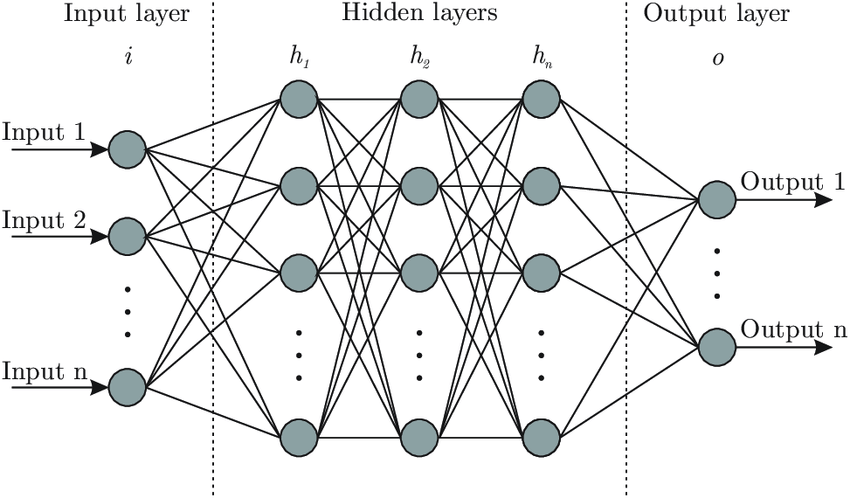
\includegraphics[width=0.8\textwidth]{Images/NN/ANN.png}
                \caption{Architettura di una rete neurale artificiale}
                \label{ANN architecture}
            \end{figure}
        
        Come mostrato nella figura \ref{ANN architecture}, l'insieme dei segnali che la ANN riceve in input si propaga attraverso gli strati intermedi, chiamati hidden layers (o strati nascosti) ed infine allo strato di output.

        \paragraph{Neurone artificiale}
        I neuroni sono gli elementi costitutivi delle reti neurali.
            \begin{figure}
                \centering
                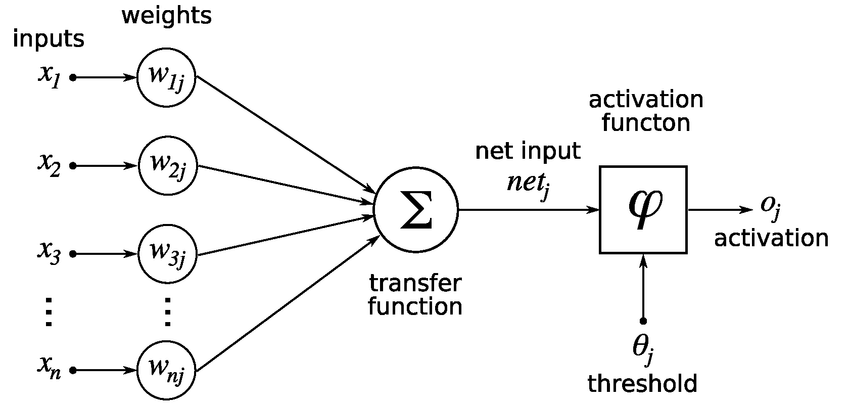
\includegraphics[width=0.7\textwidth]{Images/NN/Neuron.png}
                \caption{Struttura di un neurone}
                \label{Neuron}
            \end{figure}
        La figura \ref{Neuron} mostra una delle strutture base di un neurone. Un insieme di valori di input sono pesati e sommati. Questo risultato è usato come input per una activation function (o funzione di attivazione) che determina quanto il neurone sarà attivato dal segnale di input ricevuto.
        
        Per questo motivo, l'analogia con il cervello umano è forte, un neurone biologico è attivato da qualche segnale di input e propaga il suo output ad altri. 
        
        Le variabili della figura \ref{Neuron} sono di seguito riportate:
            \begin{itemize}
                \item $x_i$: è uno dei valori in input
                \item $w_i$: è uno dei pesi
                \item $\theta$: è la soglia di attivazione
            \end{itemize}
        
        \paragraph{Algoritmo di retropropagazione}
        L'algoritmo di back propagation (o retropropagazione) è un algoritmo di apprendimento delle reti neurali. L'algoritmo confronta il valore in output della ANN con il valore desiderato (obiettivo). Sulla base della differenza così calcolata (errore), l'algoritmo modifica i pesi sinaptici della rete neurale, facendo convergere progressivamente il set dei valori di output verso quelli desiderati.
        
    \newpage    
    \subsection{Convolutional Neural Networks (CNN)}
        
        \paragraph{Cos'è una rete neurale convoluzionale?}
        Una Convolutional Neural Network (o rete neurale convoluzionale) è una classe di reti neurali specializzata nell'elaborazione di dati che hanno una topologia a griglia, come un'immagine.\\
            \begin{figure}[!h]
                \centering
                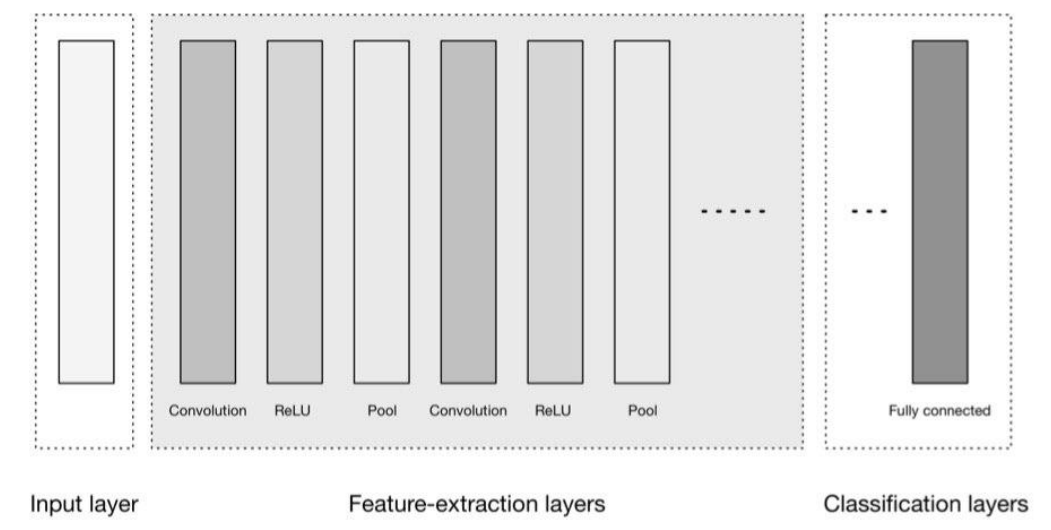
\includegraphics[width=0.8\textwidth]{Images/NN/CNN.png}
                \caption{Panoramica ad alto livello della struttura di una CNN}
                \label{CNN architecture}
            \end{figure}
        
        La figura \ref{CNN architecture} mostra una panoramica ad alto livello dell'organizzazione di una CNN. Oltre allo strato di input, gli strati intermedi realizzano l'estrazione delle caratteristiche mentre la parte finale completamente connessa esegue la classificazione.
        
        Nelle architetture CNN di base, l'estrazione delle caratteristiche viene eseguita con uno schema ripetuto. Prima, l'input attraversa uno strato di convoluzione, poi viene applicata una funzione di attivazione (generalmente la ReLU) e, infine, passa per uno strato di pooling, che riduce la dimensione delle informazioni.
        
        \paragraph{Convolution Layer}
        Il Convolutional layer (o strato di convoluzione) è il blocco fondamentale della CNN. Il suo ruolo è quello di trovare la congiunzione locale tra le caratteristiche degli strati precedenti.
        
        I weights (o pesi) in una rete neurale convoluzionale sono raggruppati in matrici chiamate kernels (o filtri).
            \begin{figure}[!h]
                \centering
                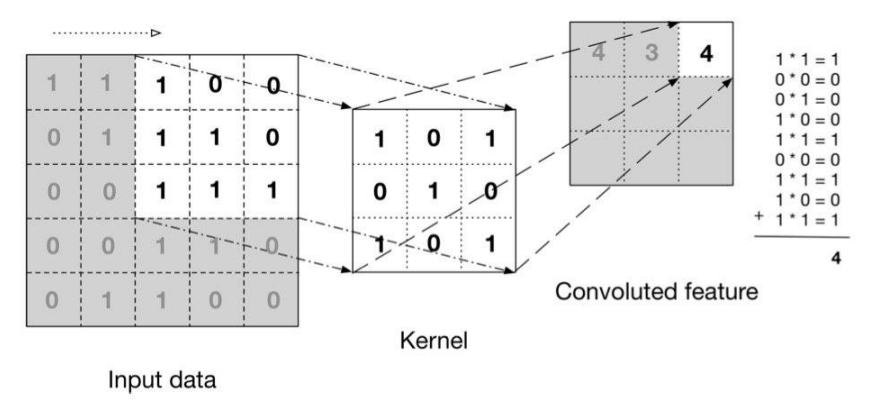
\includegraphics[width=0.7\textwidth]{Images/NN/Convolutional Layer.png}
                \caption{Operazione di convoluzione}
                \label{Convolution}
            \end{figure}
        
        \newpage
        Come mostrato in figura \ref{Convolution} l'operazione di convoluzione viene applicata moltiplicando un kernel per un'area dell'immagine di input (ogni valore viene moltiplicato per il peso corrispondente, quindi il risultato è la somma di tutte le moltiplicazioni). Il risultato viene memorizzato nella matrice di output chiamata mappa delle caratteristiche o mappa di attivazione. Ci sono molti di questi kernels. Una volta che l'input è stato completamente elaborato, la rete utilizza il kernel successivo. 
        
        È importante notare che la profondità della mappa di attivazione non è legata all'input o alla profondità del kernel, ma è uguale al numero di kernel applicati all'immagine di input.\\
        
        Alcune definizioni per questo strato:
            \begin{itemize}
                \item N: larghezza/altezza dell'input, nel caso semplificato di un'immagine di input quadrata.
                \item P: la quantità di padding usata nell'input. Il padding è utile per ottenere una dimensione desiderata nella mappa di attivazione, per esempio, per mantenere le stesse dimensioni dell'input.
                \item S: lo stride. Esprime di quanto viene spostato un kernel durante la convoluzione.
                \item F: la dimensione del kernel.
            \end{itemize}
        
        La dimensione della mappa delle caratteristiche di output è: 
            \begin{equation}
                \left\lfloor\frac{N + 2P - F}{S}\right\rfloor + 1
            \end{equation}

        \paragraph{Pooling Layer}
        Il Pooling Layer (o strato di pooling) raggruppa caratteristiche semanticamente simili trovate nella precedente mappa di attivazione e aiuta a controllare l'overfitting.
        
        Gli strati di pooling più comuni sono il Max-pooling layer, che estrae il valore massimo, e il Average-pooling layer, che calcola la media dei valori.
            \begin{figure}[!h]
                \centering
                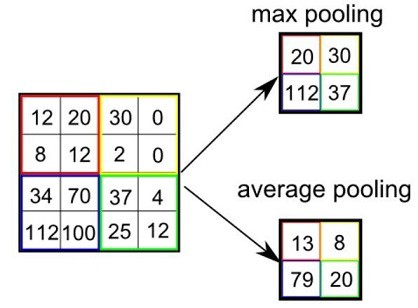
\includegraphics[width=0.3\textwidth]{Images/NN/Pooling Layer.jpeg}
                \caption{Esempio di Max-pooling e Average-pooling.
                I diversi colori evidenziano diverse aree dell'input allo strato di polling.}
                \label{Pooling}
            \end{figure}
        
        \paragraph{Fully Connected Layer}
        Il Fully Connected Layer (o strato completamente connesso) prende l'output dello strato di convoluzione/pooling, lo appiattisce e predice la migliore etichetta per descrivere l'immagine. Come in una normale rete neurale feed-forward, gli ingressi allo strato completamente connesso sono moltiplicati per i pesi e sommati insieme. Poi viene utilizzata una funzione di attivazione  per produrre l'output. I risultati sono propagati allo strato successivo completamente connesso. L'ultimo ha un neurone per ogni etichetta di classe e produce la distribuzione di probabilità.

        \paragraph{Non-Linearity Layers}
        Poiché la convoluzione è un'operazione lineare e le immagini sono tutt'altro che lineari, i Non-Linearity Layers (o strati di non linearità) sono spesso posti direttamente dopo lo strato di convoluzione per introdurre la non linearità nella mappa di attivazione.\\
        
        Ci sono diversi tipi di operazioni non lineari, le più popolari sono:
            \begin{itemize}
                \item \textbf{Sigmoid}: funzione che prende un numero reale e lo standardizza in un intervallo tra 0 e 1.\\
                    \begin{center}
                        \resizebox{8cm}{!} {
                            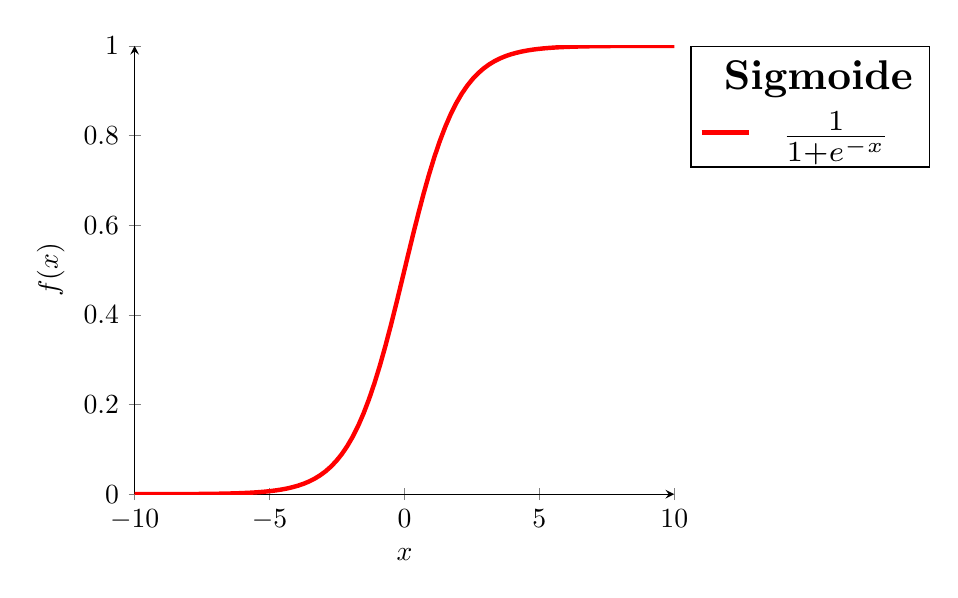
\begin{tikzpicture}
                                \begin{axis}[
                                    axis lines = left,
                                    xlabel = \(x\),
                                    ylabel = {\(f(x)\)},
                                    legend pos=outer north east,
                                    legend style={nodes={scale=1.5, transform shape}}
                                ]
                                \addlegendimage{empty legend}
                                \addplot [
                                    domain=-10:10, 
                                    samples=100, 
                                    color=red,
                                    ultra thick,
                                ]
                                {1/(1+e^(-x))};
                                
                                \addlegendentry{\hspace{-.3cm}\textbf{Sigmoide}}
                                \addlegendentry{$\frac{1}{1+e^{-x}}$}
                                \end{axis}
                            \end{tikzpicture}
                        }
                    \end{center}
                \item \textbf{Tanh}: funzione che prende un numero reale e lo standardizza in un intervallo tra -1 e 1.\\
                    \begin{center}    
                        \resizebox{8cm}{!} {
                            \begin{tikzpicture}
                                \begin{axis}[
                                    axis lines = left,
                                    xlabel = \(x\),
                                    ylabel = {\(f(x)\)},
                                    legend pos=outer north east,
                                    legend style={nodes={scale=1.5, transform shape}}
                                ]
                                \addlegendimage{empty legend}
                                \addplot [
                                    domain=-10:10, 
                                    samples=100, 
                                    color=red,
                                    ultra thick,
                                ]
                                {tanh(x)};
                                
                                \addlegendentry{\hspace{-.3cm}\textbf{Tanh}}
                                \addlegendentry{$\tanh{x}$} 
                                \end{axis}
                            \end{tikzpicture}
                    }
                    \end{center}
                \item \textbf{Rectified Linear Unit (ReLU)} 
                    \begin{center}    
                        \resizebox{8cm}{!} {
                            \begin{tikzpicture}
                                \begin{axis}[
                                    axis lines = left,
                                    xlabel = \(x\),
                                    ylabel = {\(f(x)\)},
                                    legend pos=outer north east,
                                    legend style={nodes={scale=1.5, transform shape}} 
                                ]
                                \addlegendimage{empty legend}
                                \addplot [
                                    domain=-10:10, 
                                    samples=100, 
                                    color=red,
                                    ultra thick,
                                ]
                                {max(0, x)};
                                
                                \addlegendentry{\hspace{-.3cm}\textbf{ReLU}}
                                \addlegendentry{$\max(0, x)$} 
                                \end{axis}
                            \end{tikzpicture}
                        }
                    \end{center}
            \end{itemize}
\newpage  
        \paragraph{Classification problem}
        Le CNN sono ritenute le reti neurali più efficienti quando si tratta di risolvere i problemi di classificazione.
        
        Per un classification problem (o problema di classificatione) a $K$-classi ($K \geq 2$), dato un dataset $\{(x_i, y_i)\}_{i=1,...,N}$ dove $x_i \in \mathbb{R}^d$ è un'immagine pulita e $y_i \in \{1, ... , K\}$ è la sua classe, un classificatore DNN $h$ con parametri $\theta$ predice la classe di un input $x_i$:
            \begin{equation}
                h(x_i) = \operatorname*{arg\,max}_{k = 1, ..., K}p_k(x_i, \theta)
            \end{equation}
        dove
            \begin{equation}
                p_k(x_i, \theta) = \frac{\text{exp}(z_k(x_i, \theta))}{\sum_{k'=1}^{K}\text{exp}(z_{k'}(x_i, \theta))}
            \end{equation}
        dove $z_k(x_i, \theta)$ è il logits output della rete rispetto alla classe $k$, e $p_k(x_i, \theta)$ è la probabilità (softmax su logits) che $x_i$ appartenga alla classe $k$. I parametri $\theta$ del modello sono aggiornati usando la back-propagation per minimizzare la classification loss.
\newpage
\section{Tecniche di Adversarial Attacks}
\label{Tecniche di Adversarial Attacks}

    \paragraph{Cos'è un adversarial attack}
    Dato un modello pre-trainato $h$ e un'immagine pulita $x$ associata ad un'etichetta di classe $y$, un metodo di attacco consiste nel massimizzare l'errore di classificazione del modello DNN, mantenendo $x_{adv}$ all'interno di una piccola \textit{$\epsilon$-ball} centrata sul campione originale $x$ $(||x_{adv}-x||_p \leq \epsilon)$, dove $||\cdot||_p$ è la $L_p$-\textit{norm}, sapendo che $L_\infty$ è la norma più utilizzata a causa della sua consistenza rispetto alla percezione umana.\\
    \newline
    Un adversarial attack può essere \textit{targeted} o \textit{untargeted}:
        \begin{itemize}
            \item Un \textbf{targeted attack} consiste nel trovare un adversarial example $x_{adv}$ che venga classificato della DNN in una classe specifica $h(x_{adv} \neq y_{target})$ diversa dalla classe reale di $x$ $(y_{target} \neq y)$
            \item Un \textbf{untargeted attack} consiste nel trovare un adversarial example $x_{adv}$ che venga classificato in modo errato della DNN in una classe arbitraria $h(x_{adv} \neq y)$
        \end{itemize}
    Un adversarial attack può essere \textit{white-box} o \textit{black-box}:
        \begin{itemize}
            \item Un \textbf{white-box attack} presume la conoscenza completa del modello attaccato, compresi i valori dei parametri, l'architettura, il metodo di addestramento e, più raramente, anche i dati utilizzati durante quest'ultimo.
            \item Un \textbf{black-box attack} alimenta un modello mirato con adversarial examples (durante i test) generati senza avere alcuna conoscenza di quel modello. 
            \item In alcuni casi, si presume che l'avversario abbia una conoscenza limitata del modello (ad esempio la sua procedura di addestramento e/o la sua architettura), ma sicuramente non conosce il modello.In altri casi, l'utilizzo di qualsiasi informazione sul modello di destinazione è indicato come \textit{semi-black-box attack}.
        \end{itemize}
    Nel documento verranno analizzati untargeted e targeted attacks in ambiente white-box sotto il vincolo di perturbazione $L_\infty$.\\ 
    \newline
    Per gli \textit{white-box untargeted attacks}, gli adversarial examples vengono generati risolvendo il seguente problema di ottimizzazione vincolata:
        \begin{equation}
            x_{adv}=\operatorname*{arg\,max}_{||x'-x||_\infty \leq \epsilon}l(h(x'),y)
        \end{equation}
        dove $l(\cdot)$ è la classification loss, e $y$ è la classe reale.\\
    \newline
    Per gli \textit{white-box targeted attacks}, gli adversarial examples vengono generati risolvendo il seguente problema di ottimizzazione vincolata:
        \begin{equation}
            x_{adv}=\operatorname*{arg\,min}_{||x'-x||_\infty \leq \epsilon}l(h(x'),y_{target})
        \end{equation}
        dove $l(\cdot)$ è la classification loss, e $y$ è la classe target diversa da quella reale.
    \newpage

    \paragraph{Attacchi} Nella seguente tabella si riportano gli attacchi considerati durante il lavoro di tesi:
        \begin{table}[!h]
            \centering
            \begin{tabular}{|c|c|c|c|c|}
                \hline
                \rule[-3mm]{0mm}{8mm}
                \textbf{Attack}   &\textbf{Target}  & \textbf{Settings} & \textbf{Perturbation Norm} & \textbf{Learning}  \\ \hline \hline
                \rule[-3mm]{0mm}{8mm}
                FGSM     & Targeted             & White-Box       & $l_\infty$        & One-shot  \\ \hline
                \rule[-3mm]{0mm}{8mm}
                BIM      & Untargeted           & White-Box       & $l_\infty$        & Iterative \\ \hline
                \rule[-3mm]{0mm}{8mm}
                PGD      & Targeted             & White-Box       & $l_\infty$, $l_2$ & Iterative \\ \hline
                \rule[-3mm]{0mm}{8mm}
                DeepFool & Untargeted           & White-Box       & $l_\infty$, $l_2$ & Iterative \\ \hline
            \end{tabular}
            \caption{Riassunto degli attributi di diversi metodi di attacco.}
            \label{Tab Attacks}
        \end{table}
    
    \subsection{Fast Gradient Sign Method (FGSM)}
    \label{FGSM}
    Goodfellow \cite{goodfellow2014explaining} sviluppò un metodo per calcolare efficientemente un adversarial perturbation data un'immagine pulita, risolvendo la seguente equazione:
        \begin{equation}
            \eta = \epsilon\, \text{sign} (\nabla_x J(\theta, x, y))
        \end{equation}
        dove $x$ è l'immagine pulita in input, $y$ è la classe reale di $x$ e $\theta$ rappresenta i pesi del modello attaccato. Inoltre, $\epsilon$ è la magnitudine della perturbazione, un valore scalare arbitrariamente piccolo che limita la norma della perturbazione, $J(\theta, x, y)$ è la gradient loss, sign$(\cdot)$ è la sign function e $\nabla_x(\cdot)$ è il gradiente rispetto ad $x$.\\
    \newline
    L'adversarial example è calcolato come segue:
        \begin{equation}
            \begin{split}
                x_{adv} &= x + \eta \\
                        &= x + \epsilon\, \text{sign} (\nabla_x J(\theta, x, y))
            \end{split}
        \end{equation}
    Il Fast Gradient Sign Method è uno dei primi attacchi proposti per la generazione di adversarial examples.
    \newpage
    \subsection{Basic Iterative Method (BIM)}
    \label{BIM}
    Un metodo \textit{one-step} perturba le immagini facendo un unico grande passo nella direzione che aumenta la \textit{loss} del classificatore. Un'estensione intuitiva di questa idea consiste nel fare, iterativamente, più piccoli passi aggiustando la direzione dopo ogni passo.
    
    Il Basic Iterative Method (BIM) \cite{kurakin2016adversarial} è un'estensione dell'attacco FGSM e consiste nel ripetere quest'ultimo più volte usando un passo di lunghezza ridotta.
    
    Invece di applicare un adversarial noise $\eta$ una singola volta con un parametro $\epsilon$, lo si applica più volte, iterativamente, con uno step-size $\alpha$ molto piccolo.\\
    
    L’adversarial example è calcolato attraverso la seguente formula ricorsiva:
        \begin{equation}
            \begin{split}
                x_{adv}^0 &= x,\\
                x_{adv}^i &= \text{clip}_{x, \epsilon}(x_{adv}^{i-1}+ \alpha\, \text{sign} (\nabla_{x_{adv}^{i-1}} J(\theta, x_{adv}^{i-1}, y)))
            \end{split}    
        \end{equation}
    dove $\text{clip}_{x, \epsilon}(\cdot)$ rappresenta un \textit{clipping} dei valori dell'adversarial example in modo che siano all'interno di un\textit{ $\epsilon$-neighborhood} dell'immagine pulita $x$.\\
    
    Questo approccio è vantaggioso perché permette un controllo maggiore sull'attacco. Ad esempio, si può controllare quanto oltre il confine di classificazione viene spinto un campione. A quel punto si può scegliere se terminare il ciclo durante la prima iterazione in cui $x_{adv}^i$ viene classificato in modo errato, oppure aggiungere rumore aggiuntivo oltre quel punto.
    
    Questi miglioramenti hanno reso l'attacco BIM più efficace rispetto a FGSM utilizzando perturbazioni minori e quindi, meno percettibili all'occhio umano.
    
    \subsection{Project Gradient Descent (PGD)}
    \label{PGD}
    L'attacco Project Gradient Descent (PGD) \cite{madry2017towards} perturba un'immagine pulita $x$ per un numero di passi $I$ di dimensioni molto piccole. Dopo ogni passo di perturbazione, l'attacco proietta di nuovo l'immagine perturbata sulla \textit{$\epsilon$-ball} di $x$.
    
    Se va oltre:
        \begin{equation}
            \begin{split}
                x_{adv}^0 &= x + \mathcal{U}^d(-\epsilon,\epsilon),\\
                x_{adv}^i &= \prod_{\epsilon}(\text{clip}_{x, \epsilon}(x_{adv}^{i-1}+ \alpha\, \text{sign} (\nabla_{x_{adv}^{i-1}} J(\theta, x_{adv}^{i-1}, y))))
            \end{split} 
        \end{equation}
    dove $\alpha$ è lo step-size, $\prod(\cdot)$ è la funzione di proiezione, e $x^i$ è l'adversarial example all'i-esimo step.
    
    Differentemente dall'attacco BIM ($x_{adv}^0 = x$), l'attacco PGD usa uno start casuale:
    $x_{adv}^0 = x + \mathcal{U}^d(-\epsilon,\epsilon)$.\\
    Dove $\mathcal{U}^d(-\epsilon,\epsilon)$ è la distribuzione uniforme tra $-\epsilon$ e $\epsilon$, della stessa dimensione $d$ di $x$.
    
    L'attacco PGD è considerato l'attacco di primo ordine più forte ed efficace.
    \newpage
    
    \subsection{DeepFool}
    \label{DeepFool}
    Moosavi-Dezfooli \cite{moosavi2015deepfool} hanno proposto di calcolare una perturbazione avversaria a norma minima per una data immagine in modo iterativo.
    
        \subsubsection*{DeepFool per classificatori binari}
        Si può facilmente dimostrare, usando un classificatore binario lineare, che la robustezza del modello $f$ per un input $x_{0}$, $\Delta(x_0;f)^2$, è uguale alla distanza di $x_{0}$ dal piano degli iperparametri $\text{\calligra F}=\{x:w^Tx+b=0\}$ (che separa le 2 classi).
        
        La minima perturbazione per cambiare la decisione del classificatore corrisponde alla proiezione ortogonale di $x_{0}$ sul piano degli iperparametri {\calligra F}.
            \begin{figure}[h!]
                \centering
                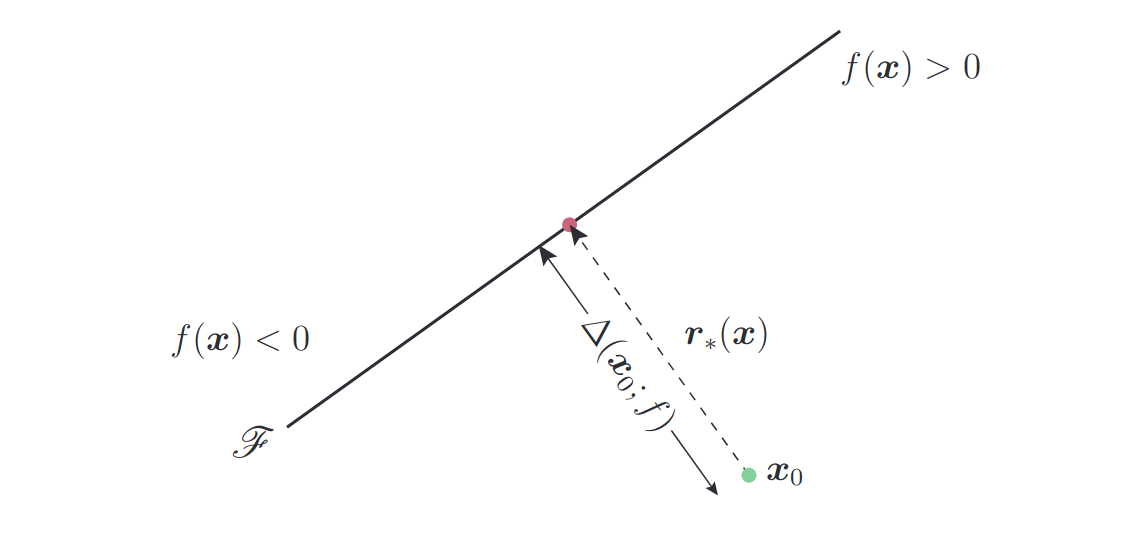
\includegraphics[width=\textwidth]{Images/DeepFool/Deepfool_1.png}
                \caption{Adversarial examples per un classificatore binario lineare}
                \label{DeepFool_1}
            \end{figure}\\
        
        La minima perturbazione è data da:
            \begin{equation}
                \begin{split}
                    r_*(x_0) :&= \operatorname*{arg\,min}_{sign(f(x_0+r)) \neq sign(f(x_0))} ||r||_2\\
                              &= -\frac{f(x_0)}{||w||_2^2}w
                \end{split}
            \end{equation}
            
        \newpage
        Di seguito è riportato l'algoritmo dell'attacco DeepFool per i classificatori binari:
            \begin{figure}[h!]
                \centering
                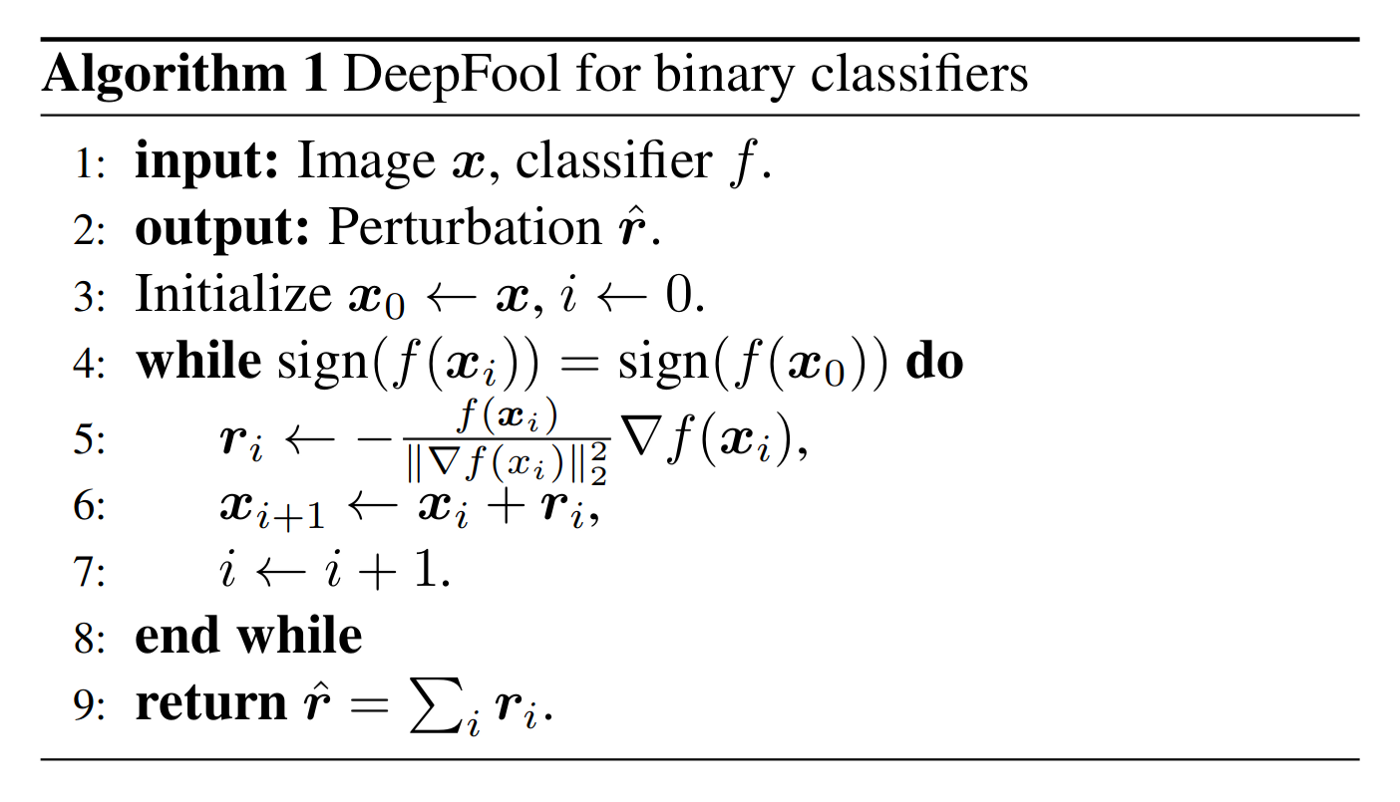
\includegraphics[width=0.8\textwidth]{Images/DeepFool/Deepfool_2.png}
                \caption{}
                \label{DeepFool_2}
            \end{figure}
            
            \paragraph{Analisi algoritmo}
                \begin{enumerate}
                    \item L'algoritmo prende in input $x$ e un classificatore $f$
                    \item Restituisce in output la perturbazione minima richiesta per classificare in modo errato l'immagine
                    \item Inizializza l'adversarial example con l'input originale. E la variabile $i$ del ciclo a 1.
                    \item Avviare il ciclo. Continuare il ciclo finché l'etichetta vera e l'etichetta dell'immagine perturbata avversariamente sono uguali.
                    \item Calcolare la perturbazione minima, ovvero la proiezione dell'input sull'iperpiano più vicino.
                    \item Aggiungere la perturbazione calcolata all'immagine e testare.
                    \item Incrementare la variabile del loop
                    \item Fine del loop.
                    \item Restituire la perturbazione minima.
                \end{enumerate}
            \newpage
        
        \subsubsection*{DeepFool per classificatori multiclasse}
        Moosavi-Dezfooli \cite{moosavi2015deepfool} descrivono un classificatore multiclasse come un insieme di classificatori binari.
        Per i classificatori multiclasse l'input è $x$ e per ogni classe c'è un iperpiano (piano rettilineo che divide una classe dalle altre) e, in base alla posizione che occupa nello spazio, $x$ viene classificato in una classe specifica.
        
        Ciò che fa l'algoritmo è trovare l'iperpiano più vicino, proiettare $x$ su quell'iperpiano e poi spingerlo oltre l'intersezione. In questo modo la classificazione di $x$ verrà sbagliata con la minima perturbazione possibile.\\
        
        Di seguito l'equazione per calcolare l'iperpiano più vicino:
            \begin{equation}
            \label{closest hyperplane}
                \hat{l}(x_0) = 
                \operatorname*{arg\,min}_{k \neq \hat{k}(x_0)} \frac{|f_k(x_0)-f_{\hat{k}(x_0)}(x_0)|}{||w_k-w_{\hat{k}(x_0)}||_2}
            \end{equation}
        dove: le varibiabili che cominciano con $f$ sono le etichette di classe, la variabili che cominciano con $w$ sono i gradienti, le variabili con $k$ come pedice sono per le classi con più probabilità dopo la classe reale, e le variabili con $\hat{k}(x_0)$ sono per la classe reale.\\
        
        Di seguito l'equazione per calcolare la perturbazione minima, ovvero il vettore che proietta l'input sull'iperpiano più vicino:
            \begin{equation}
            \label{minimal perturbation}
                r_*(x_0)=\frac{|f_{\hat{l}(x_0)}(x_0)-f_{\hat{k}(x_0)}(x_0)|}{||w_{\hat{l}(x_0)}-w_{\hat{k}(x_0)}||^2_2}(w_{\hat{l}(x_0)}-w_{\hat{k}(x_0)})
            \end{equation}\\
        
        Di seguito è riportato l'algoritmo dell'attacco DeepFool per i classificatori multiclasse:
            \begin{figure}[h!]
                \centering
                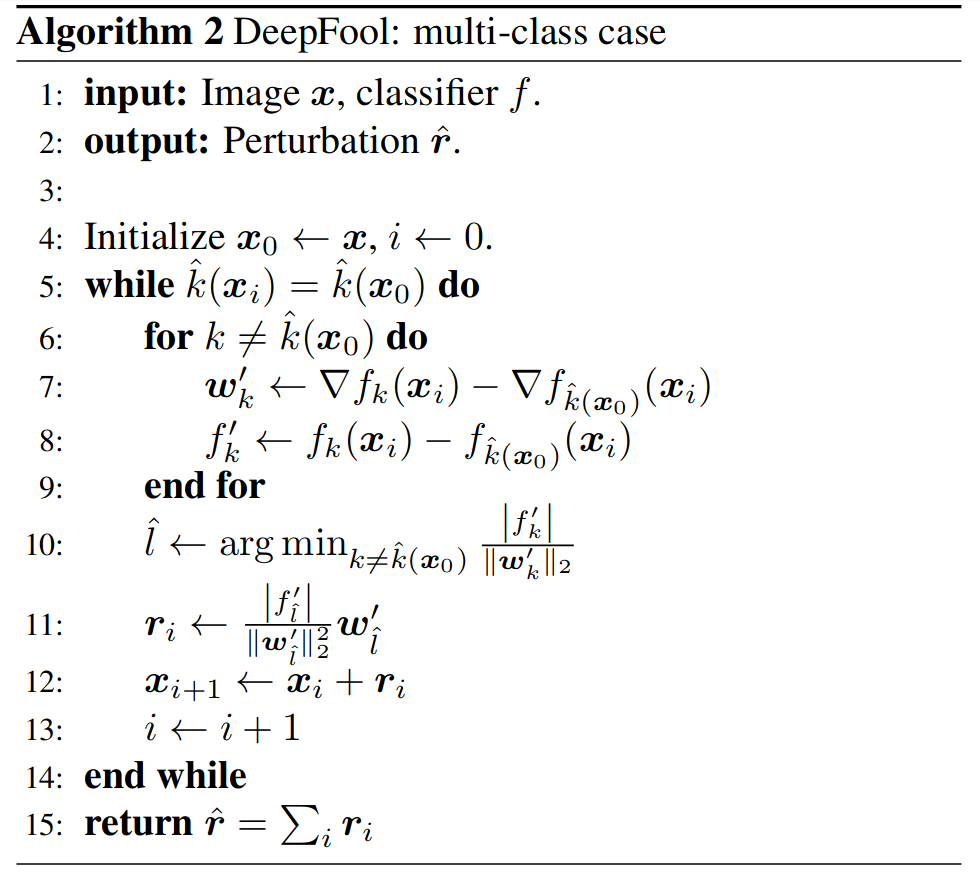
\includegraphics[width=0.7\textwidth]{Images/DeepFool/Deepfool_3.png}
                \caption{}
                \label{DeepFool_3}
            \end{figure}
        
            \paragraph{Analisi algoritmo}
                \begin{enumerate}
                    \item L'algoritmo prende in input $x$ e un classificatore $f$
                    \item Restituisce la perturbazione 
                    \item ...
                    \item Inizializza l'adversarial example con l'input originale. E la variabile $i$ del ciclo a 1.
                    \item Avviare il ciclo. Continuare il ciclo finché l'etichetta vera e l'etichetta dell'immagine perturbata sono uguali.
                    \item Si considerino n classi che hanno avuto una probabilità maggiore dopo la classe originale:
                    \item Memorizzare la differenza minima tra i gradienti originali e i gradienti di ciascuna di queste classi $w'_k$.
                    \item Memorizzare la differenza nelle etichette $f'_k$.
                    \item ...
                    \item Utilizzare $w'_k$ e $f'_k$ per calcolare l'iperpiano più vicino $\hat{l}$ per l'input $x$. Vedi formula \ref{closest hyperplane}
                    \item Calcolare il vettore minimo $r_i$ che proietta $x$ sull'iperpiano più vicino $\hat{l}$.\\
                    Vedi formula \ref{minimal perturbation}
                    \item Aggiungere la perturbazione minima all'immagine e controllare se è stata classificata in modo errato.
                    \item Incrementare la variabile del loop
                    \item Fine del loop.
                    \item Restituire la perturbazione totale, ovvero la somma di tutte le perturbazioni calcolate.
                \end{enumerate}
            \newpage
    
\section{Tecniche di Mitigation di Adversarial Attacks}
\label{C3: Mitigation}
    \begin{figure}[!h]
        \centering
        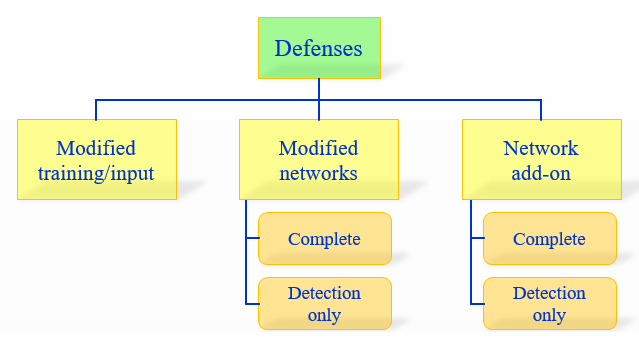
\includegraphics[width=0.8\textwidth]{Images/Mitigation/Defenses.png}
        \caption{Ampia categorizzazione di approcci volti a difendere le DNN dagli adversarial attacks.}
        \label{Defenses}
    \end{figure}
    Attualmente, le difese contro gli adversarial attacks si stanno sviluppando lungo 3 direzioni principali %[bibl: https://engineering.virginia.edu/sites/default/files/common/departments/electrical-and-computer-engineering/computer-engineering/files/Threat%20of%20Adversarial%20Attacks.pdf]
    \cite{akhtar2018threat}:
        \begin{enumerate}
            \item Modificare il metodo di apprendimento durante la fase di training o gli input durante la fase di testing.
            \item Modificare la rete, ad esempio aggiungendo più strati/sottoreti, cambiando loss function o activation function, ecc.
            \item Usando modelli esterni come network add-on quando si classificano esempi mai visti.
        \end{enumerate}
    Nel primo caso non ci si occupa direttamente del modello di apprendimento. Al contrario, le altre due categorie sono più incentrate sulle reti neurali stesse. In particolare:
        \begin{itemize}
            \item \textbf{Modifica di una rete}: si apportano modifiche all'architettura e/o ai parametri della rete neurale originale durante la fase di training.
            \item \textbf{Network add-on}: si mantiene il modello originale intatto e si aggiungono uno o più modelli esterni durante la fase di testing. Questi ultimi vengono utilizzati per preprocessare gli input prima che vengano passati al modello originale.
        \end{itemize}
    Le tecniche sotto queste categorie possono essere ulteriormente divise in due tipi: 
        \begin{itemize}
            \item \textbf{Complete defence} (Difesa completa): approccio che mira a permettere al modello attaccato di svolgere il suo compito originale anche sugli adversarial examples. Nel caso di un classificatore, ci si aspetta che il modello predica le classi degli adversarial examples con una precisione accettabile.
            \item \textbf{Detection only} (Solo rilevamento): approccio che mira ad individuare i potenziali adversarial examples, per poterli contrassegnare e rifiutare in qualsiasi elaborazione futura.
        \end{itemize}
    La gerarchia di queste categorie è mostrata nella figura \ref{Defenses}.
    Il resto della sezione è organizzato secondo questa gerarchia.
    \newpage
    
    \subsection{Modified Training/Input}
    \label{BF Adversarial Training}    
        \subsubsection{Brute-force adversarial training}
        L'adversarial training %[bibl: https://arxiv.org/pdf/1412.6572.pdf] 
        \cite{goodfellow2014explaining} è un metodo di difesa intuitivo contro gli adversarial attacks, che cerca di migliorare la robustezza di una rete neurale trainandola con adversarial examples.
        
        Formalmente, può essere formulato come segue:
            \begin{equation}
                \operatorname*{min}_{\theta} \operatorname*{max}_{D(x, x_{adv})<\eta}J(\theta,x_{adv},y)
            \end{equation}
        dove $J(\theta,x_{adv},y)$ è l'\textit{adversarial loss}, con \textit{weights} $\theta$, \textit{adversarial input} $x_{adv}$, e classe reale $y$. $D(x, x_{adv})$ è la distanza tra $x$ e $x_{adv}$.
        Il problema di massimizzazione interna è quello di trovare gli adversarial examples più efficaci ed è risolto da un adversarial attack ben progettato, come FGSM (\hyperref[FGSM]{\ref*{FGSM}}) e PGD (\hyperref[PGD]{\ref*{PGD}}).  
        La minimizzazione esterna è la procedura di addestramento standard per minimizzare la \textit{loss}. 
        
        Risolti i problemi di massimizzazione e minimizzazione, si suppone che la rete risultante sia resistente contro l'adversarial attack usato per la generazione di adversarial examples nella fase di training.
        
        Anche se l'adversarial training migliora la robustezza di una rete, è una strategia non adattativa che richiede che il training sia eseguito utilizzando attacchi forti e che l'architettura della rete sia sufficientemente rappresentativa.
        Inoltre, il metodo richiede un raddoppio della dimensione del Training dataset e, di conseguenza, un aumento di tempo e risorse investite nella fase di training.
            \begin{figure}[!h]
                \centering
                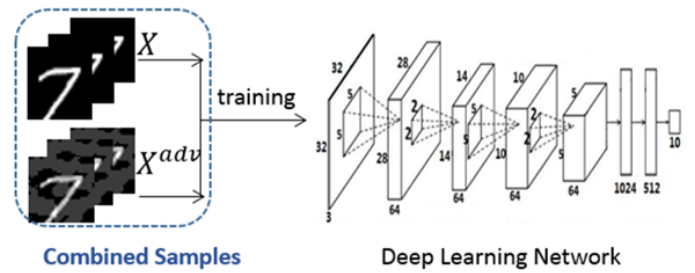
\includegraphics[width=0.8\textwidth]{Images/Mitigation/Adversarial training.png}
                \caption{Adversarial Training: trainare il modello con immagini pulite e perturbate}
                \label{Adversarial Training}
            \end{figure}
    \newpage
    
        \subsubsection{Random input transformation}
        In %[bibl: https://arxiv.org/pdf/1711.01991.pdf]
        \cite{xie2017mitigating} gli autori utilizzano due trasformazioni casuali per mitigare gli effetti degli adversarial attacks:
            \begin{enumerate}
                \item \textbf{Random resize}: ridimensionamento delle immagini di input ad una dimensione casuale prima di passarle alla rete neurale. 
                \item \textbf{Random padding}: riempimento con degli zeri intorno alle immagini di input in modo casuale.
            \end{enumerate}
        La pipeline di questo meccanismo rapido e preciso è mostrata nella figura \ref{Random resize and padding}
            \begin{figure} [!h]
                \centering 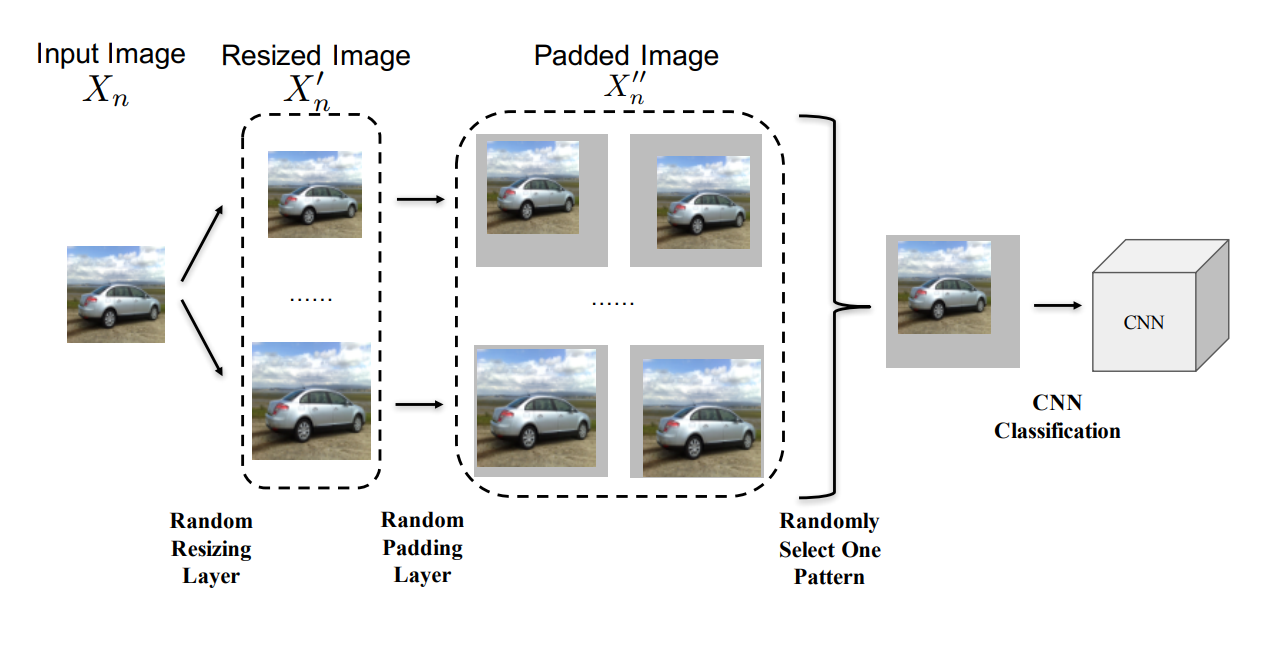
\includegraphics[width=\textwidth]{Images/Mitigation/Random resize and padding.png}
                \caption{Pipeline del meccanismo di difesa basato sulla randomizzazione. L'immagine in input $X_n$ passa attraverso il random resize layer che la scala in modo casuale. Poi, il random paddding layer applica il padding all'immagine ridimensionata $X'_n$ in maniera casuale. L'immagine risultante $X''_n$ viene utilizzata per la classificazione}
                \label{Random resize and padding}
            \end{figure}
    \newpage
    
    
    
    \subsection{Modified Networks}
        
        \subsubsection{Random noising}
        Random self-ensemble (RSE) %[bibl: https://arxiv.org/pdf/1712.00673v2.pdf]
        \cite{liu2017towards} è un algoritmo che aggiunge un noise layer dopo ogni convolutional layer in entrambe le fasi di training e testing, e raggruppa i risultati delle predizione per stabilizzare gli output della rete neurale, come mostrato nella Figura \ref{Random noising}.
        
        Lo stesso metodo può essere sviluppato utilizzando la differential privacy (DP). Il metodo PixelPD 
        %[bibl: https://ieeexplore.ieee.org/stamp/stamp.jsp?tp=&arnumber=8835364]
        \cite{lecuyer2018certified} include un DP noising layer all'interno della rete neurale per far rispettare i limiti DP sulla variazione della distribuzione sulle sue previsioni degli input con piccole perturbazioni basate sulle norme.
        
        Ispirandosi a PixelDP, Li %[bibl: https://proceedings.neurips.cc/paper/2019/file/335cd1b90bfa4ee70b39d08a4ae0cf2d-paper.pdf]
        \cite{li2018certified} propone inoltre di aggiungere direttamente del random noise ai pixel degli adversarial examples prima della classificazione, al fine di eliminare gli effetti delle perturbazioni avversarie.
            \begin{figure}[!h]
                \centering 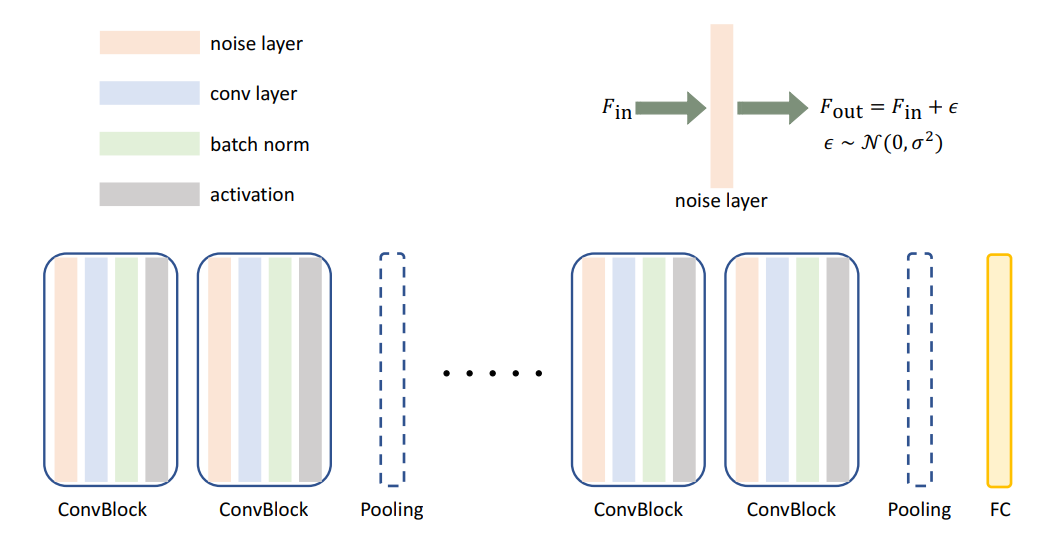
\includegraphics[width=0.8\textwidth]{Images/Mitigation/Random noising.png}
                \caption{Architettura di RSE. FC: fully connected layer; $F_in$: il vettore in input del noise layer; $F_out$: il vettore in output del noise layer; $\epsilon$: la perturbazione che segue la distribuzione gaussiana $\mathcal{N}(0, \sigma^2)$; conv: convolution}.
                \label{Random noising}
            \end{figure}
        
        \subsubsection{Gradient regularization/masking}
        In %[bibl: https://arxiv.org/pdf/1711.09404.pdf]
        \cite{ross2017improving} gli autori propongono un metodo che traina modelli differenziabili (ad esempio DNN) penalizzando il grado di variazione che risulta in output rispetto al cambiamento in input. Applicando una piccola perturbazione avversaria diventa improbabile che cambi drasticamente l'output del modello addestrato. 
        
        Si dimostra che questo metodo, quando combinato con il brute-force adversarial training, può garantire un'ottima robustezza alle reti neurali contro adversarial attacks come FGSM (\hyperref[FGSM]{\ref*{FGSM}}). 
        
        Tuttavia, ognuno di questi metodi quasi raddoppia la complessità di formazione di una rete, che risulta già proibitiva in molti casi.
    
    \newpage
    \subsection{Network Add-On}
    
        %\subsubsection{Feature Squeezing}
        %[bibl: https://arxiv.org/pdf/1704.01155.pdf] - molto vulnerabile, lo spiego comunque?
        
        \subsubsection{APE-GAN}
        Adversarial Perturbation Elimination GAN (APE-GAN) %[bibl: https://arxiv.org/pdf/1707.05474.pdf] 
        \cite{shen2017ape} ha l'obiettivo di mitigare l'adversarial attack agendo sull'input della rete neurale. 
        Sfrutta le proprietà delle GAN e la loro capacità di stimare la distribuzione dei campioni in input.
        
        APE-GAN è trainata in un ambiente avversario. Il suo Generator G, presa in input un'immagine perturbata, la restituisce in output pulita. Il suo Discriminator D confronta l'output del Generator con gli input reali puliti.
        
        In un ambiente ideale, il Generator impara a generare immagini pulite molto simili a quelle reali, rendendo difficile per il Discriminator predire la fonte delle sue immagini in input.
        \begin{figure}[!h]
            \centering
            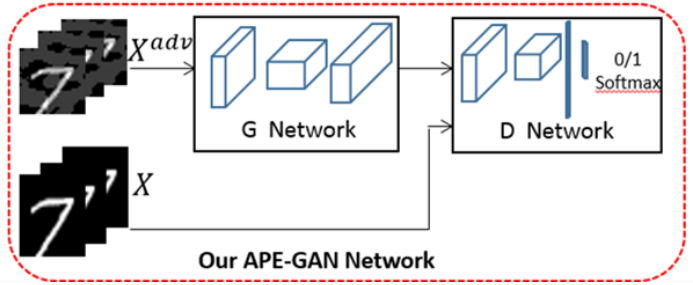
\includegraphics[width=0.6\textwidth]{Images/Mitigation/APE-GAN.png}
            \caption{APE-GAN: elimina la perturbazione dagli adversarial examples prima di passarli in input al modello originale per poterne incrementare la robustezza.}
            \label{APE-GAN}
        \end{figure}
        
        \subsubsection{Defense-GAN}
        Defense-GAN %[bibl: https://arxiv.org/pdf/1805.06605.pdf] 
        \cite{samangouei2018defense} si basa sulla tipica struttura delle WGAN %[bibl: https://arxiv.org/pdf/1701.07875.pdf]
        \cite{arjovsky2017wasserstein}. 
        
        Il Generator della Defense-GAN dovrebbe imparare a creare una mappatura da un vettore $z$ di bassa dimensione ad uno spazio di campioni di input di dimensione superiore.
        
        L'idea è di addestrare la Defence-GAN su dati originali e puliti che ci permettano di assumere con sicurezza che questi saranno vicini a qualche punto nell'intervallo di G. Ciò significa che gli adversarial examples saranno più lontani dall'intervallo di G. 
        
        Quindi, proiettare gli adversarial examples sull'intervallo del Generator si rivela un modo per diminuire le perturbazioni dalle immagini.
        
        Questo output proiettato viene dato in input alla rete neurale al posto degli adversarial examples.
            \begin{figure}[!h]
                \centering 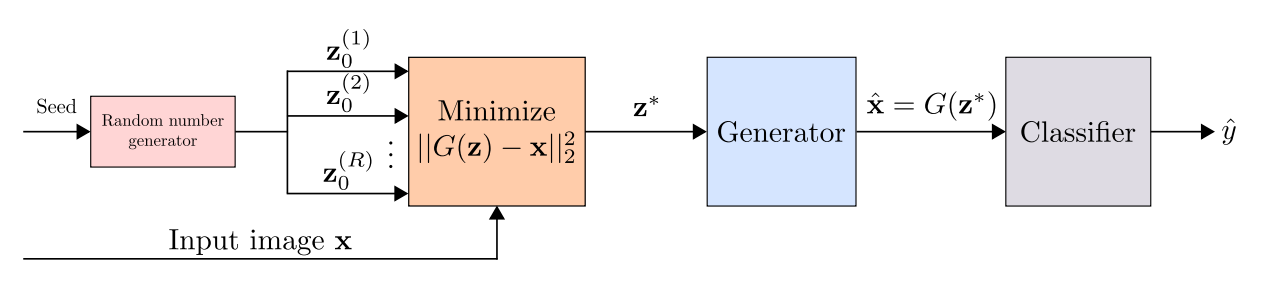
\includegraphics[width=0.9\textwidth]{Images/Mitigation/Defense-GAN.png}
                \caption{Panoramica dell'algoritmo Defense-GAN}
                \label{Defense-GAN}
            \end{figure}
        \newpage
        
        \subsubsection{MagNet}
        L'obiettivo di MagNet %[bibl: https://arxiv.org/pdf/1705.09064.pdf] 
        \cite{meng2017magnet} è quello di riconoscere gli adversarial examples.
        
        Se l'input è ritenuto pulito, MagNet lo trasforma ulteriormente con lo scopo di risolvere eventuali errori di classificazione del modello (figura \ref{MagNet}).
        
        L'architettura di MagNet consiste in un Detector e un Reformer. Entrambi possono essere costituiti da una o più reti concatenate.\\
        
        Sono stati proposti due Detectors:
            \begin{itemize}
                \item Il primo Detector sfrutta un AutoEncoder che viene trainato su campioni puliti e, quindi, impara a ricostruire le immagini appartenenti alla stessa distribuzione. Un adversarial example non apparterrà alla stessa distribuzione delle immagini pulite. Quindi, l'autoencoder trainato sulle immagini pulite avrà un'alta reconstruction loss nel caso di un adversarial example.
                \item Il primo Detector funziona bene con i campioni che hanno un elevato reconstruction error. Tuttavia non è necessario che un adversarial example abbia un elevato reconstruction error.
                
                Per questo motivo si decide di utilizzare il classificatore di destinazione. 
                
                Sia $f$ il classificatore e $ae$ l'autoencoder. Se un campione in input è perturbato, allora $f(x)$ e $f(ae(x))$ saranno molto diversi e avranno una divergenza grande.
                Si sfrutta quindi la divergenza di Jensen Shannon tra $f(x) e$ e $f(ae(x))$ per decidere se il campione in input è perturbato o pulito.
            \end{itemize}
        I Detectors sopra citati sono usati in serie con il Reformer 1 seguito dal Reformer 2. Se entrambi i Detectors ritengono l'input pulito, allora lo passano al Reformer 1:
            \begin{itemize}
                \item Reformer 1 basato sul random noise: aggiunge, all'immagine in input, un random noise basato su una distribuzione gaussiana standard. Lo svantaggio di questo reformer è che funziona allo stesso modo sia per un adversarial example che per un'immagine pulita.
                \item Reformer 2 basato su AutoEncoder: utilizza un autoencoder addestrato completamente su immagini pulite. Quando un adversarial example viene dato in input all'autoencoder, questo cercherà di ricostruire un'immagine pulita.
            \end{itemize}
        
            \begin{figure}[!h]
                \centering
                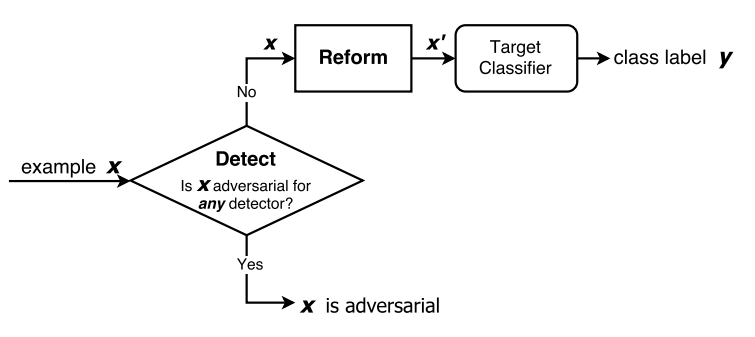
\includegraphics[width=0.7\textwidth]{Images/Mitigation/MagNet.png}
                \caption{Panoramica dell'algoritmo di MagNet}
                \label{MagNet}
            \end{figure}
    
        \subsubsection{Pix2Pix GAN}
        \label{Pix2Pix GAN}
        Una Pix2Pix GAN %[bibl: https://arxiv.org/pdf/1611.07004.pdf] 
        \cite{isola2016image} è una conditional GAN (cGAN) %[bibl: https://arxiv.org/pdf/1411.1784.pdf] 
        \cite{mirza2014conditional} ed utilizza solamente dati reali, rumore ed etichette per imparare a generare immagini.
        
        Uno dei campi in cui viene impiegata la Pix2Pix GAN è l'image denoising, ovvero, presa un'immagine che si presume perturbata con del rumore, si cerca di pulirla e riportarla allo stato originale.\\\\
        Il Generator impara la mappatura dai dati reali e dal rumore.
            \begin{equation*}
                G:\left \{ x, z \right \} \rightarrow y
            \end{equation*}
        Il Discriminator impara a la mappatura dalle etichette e dai dati reali.
            \begin{equation*}
                D(x, y)
            \end{equation*}
        Questa soluzione permette ad una cGAN di essere adatta a compiti di traduzione image-to-image, dove il Generator è vincolato ad un'immagine in input per generare un'immagine corrispondente in output. In altre parole, il Generator utilizza una condition distribution come una guida per generare un'immagine di destinazione. \\\\
        Pix2Pix GAN fonda la sua forza sulla fase di training, che consiste in una traduzione pair to pair image e il dataset utilizzato è composto da campioni di training {x, y} che hanno una corrispondenza tra loro. \\\\
        L'architettura di Pix2Pix GAN è composta da un Generator e un Discriminator:
            \begin{itemize}
                \item U-Net Generator %[bibl: https://arxiv.org/pdf/1505.04597.pdf]:
                      \cite{ronneberger2015u}:
                    \begin{figure}[!h]
                        \centering 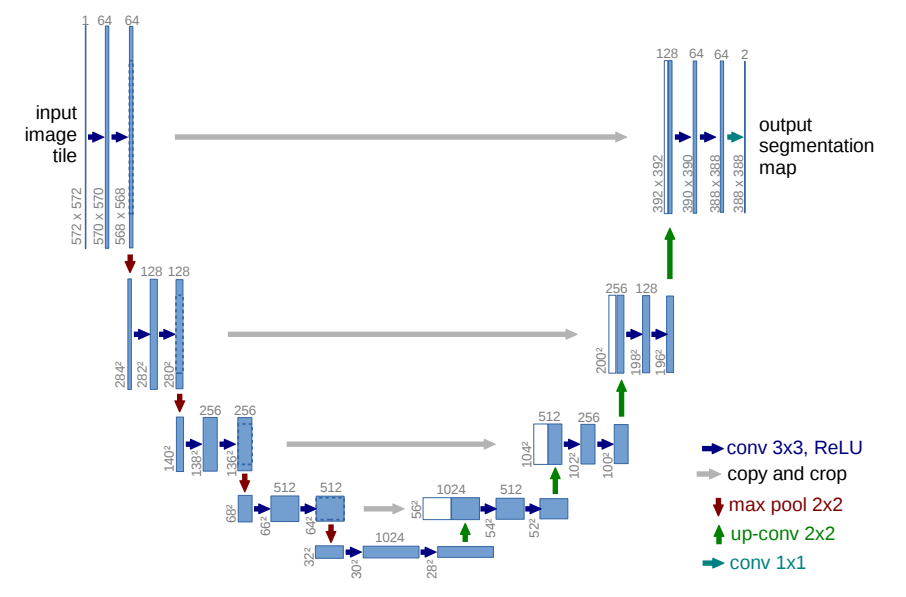
\includegraphics[width=0.8\textwidth]{Images/Mitigation/U-Net_1.png}
                        \caption{Architettura U-Net (esempio per immagini $32\times32$). \\
                        Ogni casella blu corrisponde ad una multi-channel feature map. Il numero di canali è indicato in cima al riquadro. La dimensione $x\times y$ è riportata sul bordo sinistro inferiore del riquadro.
                        I riquardi bianchi rappresentano feature maps copiate. 
                        Le frecce denotano le diverse operazioni.}
                        \label{U-Net_1}
                    \end{figure}
                \newpage
                
                U-Net si può dividere in due parti fondamentali (figura \ref{U-Net_2}):
                    \begin{enumerate}
                        \item Contracting path: è composto da convolutional layers (lato sinistro della figura \ref{U-Net_2}) che applicano un downsampling sui dati mentre estrae informazioni.
                        
                        Durante il downsampling, ogni convolutional block estrae delle informazioni parziali e le passa al convolutional block successivo per estratte ulteriori informazioni, fino a che non si raggiunge la parte centrale detta bottleneck.
                        \item Expansive path: è composto da transpose convolution layer (lato destro della figura \ref{U-Net_2}) che applica un upsampling sulle informazioni estratte in precedenza.
                        
                        L'upsampling comincia dal bottleneck.
                        Durante l'upsampling ogni transpose convolutional block espande le informazioni prese dal blocco precedente e le concatena a quelle estratte dal blocco corrente. Concatenando informazioni, U-Net può quindi imparare ad elaborare un output più preciso basandosi su queste informazioni.
                    \end{enumerate}
                    Il downsampling e l'upsampling devono avere lo stesso numero di convolution layer e transpose convolution layer. Questo perché bisognerà collegare i blocchi corrispondenti delle stesse dimensioni usando una skip connection.
                        \begin{figure}[!h]
                            \centering 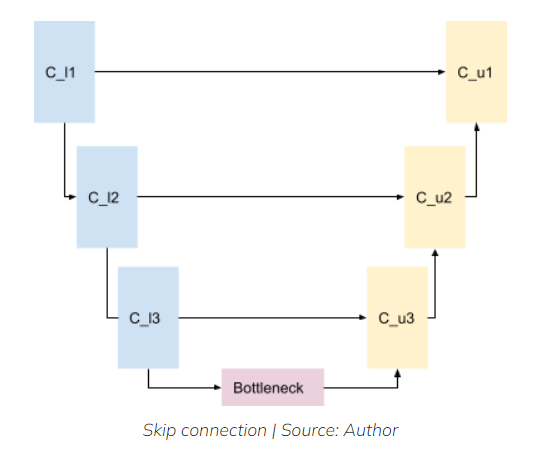
\includegraphics[width=0.7\textwidth]{Images/Mitigation/U-Net_2.png}
                            \caption{U-Net: contractive and expanding paths.}
                            \label{U-Net_2}
                        \end{figure}
                \newpage
                
                \item Markovian discriminator (PatchGAN):
                architettura contenente un certo numero di transpose convolutional blocks. Prende una porzione $N\times N$ dell'immagine e cerca di capire se è pulita o perturbata.
            
                $N$ può evere qualsiasi dimensione. $N$ può essere anche più piccolo dell'immagine originale, riuscirà comunque a produrre risultati di alta qualità.
                
                Seguendo questa procedura, il Discriminator viene applicato convoluzionalmente su tutta l'immagine. 
            \end{itemize}
        %L'equazione della loss function è la seguente ed ha due componenti, una per il Discriminator D e una per il Generator G:
        %    \begin{equation}
        %        \mathcal{L}_{cGAN}(G, D) = \mathbb{E}_{x,y}[log\, D(x, y)] + \mathbb{E}_{x,z}[log(1 - D(x, G(x, z))]
        %    \end{equation}
        
        %In ogni iterazione della fase di training della GAN il Discriminator è trainato prima del Generator in modo che possa riconoscere sia i dati reali che quelli generati dal Generator.
    \newpage